\section{Project management}
%Include a timetable (in 2 week chunks) for the remainder of the academic year, up until the submission deadline. What has been achieved, and was it expected?
The progress made so far has been mixed - some objectives have been achieved much faster than was expected, while other objectives have taken a significantly longer amount of time than expected. This has been tracked effectively using the Trello\footnote{https://trello.com/} board, and allowed for the project supervisor to be updated frequently as to how the project has been progressing. Project meetings have occurred most weeks and have been useful in informing the project supervisor of progress, as well as getting advice for any issues that arose during the week.

The initial design of the SoC took only a single week, far under the initial estimate. This was mostly due to underestimating the capabilities of the RocketChip generator. Verifying and testing the design is ongoing, as difficulty has been had in creating software that will run on the SoC after implementation on the FPGA. There has been a much smaller amount of time available for the project than planned for, and has lead to unsatisfactory progress. To rectify this, the scope has been adjusted to better fit what is possible in the remaining time, and to fit the constraints of what is known to be possible now more is known of the subject area. In addition, much more work will be complete over the December period. Several weeks were allocated to be free or have minimal work complete, but will now be used to achieve progress that should've been made previously.

Due to the issues with obtaining an FPGA that would allow mainstream Linux to be tested, the project objectives have changed so the embedded Linux is the target instead. The objective for running embedded Linux has also been moved to 'could' in figure \ref{fig:objectives}, indicating that there is a medium likelihood this objective will not be completed.

\newgeometry{left=1cm,bottom=1cm}
\begin{landscape}
    \begin{figure}[]
        \centering
        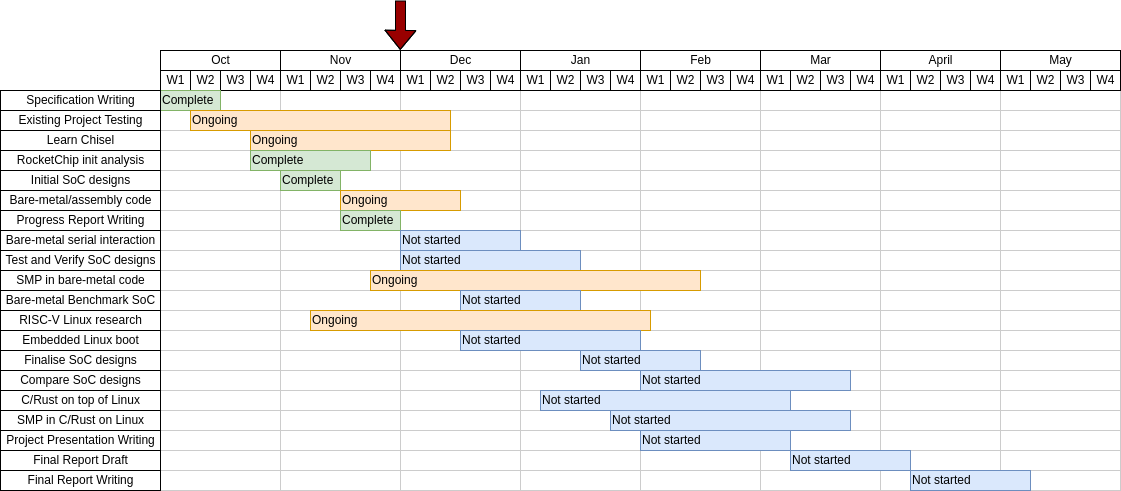
\includegraphics[scale=0.6]{./img/Gantt progress report.drawio.png}
        \caption{Gantt chart for progress tracking}
        \label{fig:Gantt}
    \end{figure}
\end{landscape}
\restoregeometry
The Gantt\cite{gantt-chart} chart in figure \ref{fig:Gantt} shows the progress that has been made so far, as well as expected tasks over the next few weeks. There is a significant amount of time between the presentation and the final report due date, and this has been left mostly empty. This is to accommodate any issues that arise during the project, and should allow time for more to be done between the presentation and report submission if necessary.